% This is samplepaper.tex, a sample chapter demonstrating the
% LLNCS macro package for Springer Computer Science proceedings;
% Version 2.20 of 2017/10/04
%
\documentclass[runningheads]{llncs}
%
\usepackage{graphicx}
\usepackage[utf8]{inputenc}
% Used for displaying a sample figure. If possible, figure files should
% be included in EPS format.
%
% If you use the hyperref package, please uncomment the following line
% to display URLs in blue roman font according to Springer's eBook style:
% \renewcommand\UrlFont{\color{blue}\rmfamily}

\begin{document}
%
\title{Versinus: an Animated Visualization Method for Evolving Networks\thanks{Supported by FAPESP}}
%
%\titlerunning{Abbreviated paper title}
% If the paper title is too long for the running head, you can set
% an abbreviated paper title here
%
\author{Renato Fabbri\inst{1}\orcidID{0000-0002-9699-629X} \and
Maria Cristina Ferreira de Oliveira\inst{1}\orcidID{0000-0002-4729-5104}}
%
\authorrunning{R. Fabbri and M. C. F. de Oliveira}
% First names are abbreviated in the running head.
% If there are more than two authors, 'et al.' is used.
%
\institute{University of São Paulo, São Carlos SP, BR\\
\email{renato.fabbri@gmail.com},
\email{cristina@icmc.usp.br}\\
\url{http://conteudo.icmc.usp.br/pessoas/cristina/}}
%
\maketitle              % typeset the header of the contribution
%
\begin{abstract}
% The abstract should briefly summarize the contents of the paper in
% 150--250 words.
Most real world networks change over time with new nodes and links or their removal, or even with metadata modification.
Increasing interest in modeling evolving networks has been reported and
a number of methods have been proposed to visualize them.  
  This article presents a novel visualization approach for (time-)evolving (or longitudinal) networks,
  specially useful for the observation of (in)stability of basic topological characteristics.
  The method has received a few software implementations and has been useful in research and publication, which motivated the writing of this present document.
  Named Versinus, the visualization consists essentially in placing the most connected nodes (hubs and intermediary) along a sine curve, and the peripheral nodes nodes along a separate segment, usually a line.
  Thus its name from  Latin \emph{versus} (line) and \emph{sinus} (sine).
  The method has provided insights into network properties and for network visualizations, which are described here after a formal presentation of the visualization and yielded software.


\keywords{Network visualization  \and Evolving networks \and Animated visualization \and Complex networks \and Data visualization.}
\end{abstract}
%
%
%
\section{Introduction}
The visualization of evolving networks poses challenges related to data size and complexity which have merited various contributions~\cite{evo1,evo2,evo3}.
In fact, the meaningful visualization of time-evolving networks is a well-known problem in information visualization (\emph{infovis}) and dynamic network analysis (\emph{DNA}).
In this work, we present a novel approach in DNA infovis that consists in distributing the nodes along a fixed layout that consists in three segments for three sections (or partitions) of a scale-free network, namely for the hub, intermediary and peripheral nodes~\cite{stab}. The development of the network is expressed by changes in node height, width, color, format, and by changes in link disposition, thickness and color. Also, auxiliary global and local information are be displayed in order to enable a sound analysis of the features of interest.
The method has been called Versinus since its early usages in 2013, because the layout stabilized, after trying many figures, in a sine period and a line, which in Latin is \emph{sinus} (sine) and \emph{versus} (line). 
Versinus has received four software implementations, two of them written in Python scripts that yield animations through stop-motion. The other two are written in JavaScript, one of them is an exploitation for static networks, the other is an ongoing Visual Analytics interface which extends the description in this document for 3D with additional analysis techniques such as principal component analysis (PCA).
The writing of this document was motivated by its usefulness in scientific research~\cite{stab,thesis} and the benefit of a careful mathematical and technological description of the procedures involved in applying the method to real networks.

The article is organized as follows. Next subsections hold remarks about related work and vocabulary. Section~\ref{sec:des} describes the method in detail and sufficient formalism. Section~\ref{sec:imp} is depicts the software implementations of Versinus. Section~\ref{sec:ins} is dedicated to revealing further insights obtained through the use of the method. Finally, Section~\ref{sec:con} convene concluding and further work commentaries.

\subsection{Related work}
% on animated visualization
% on vis of evo nets
Although animation is often criticized in the data visualization canonical literature~\cite{munzner,ware}, advantages have also been reported~\cite{cog,anim} e.g. making visuallizations more eye catching and due to the fact that we are accustumed to moving through the world and to moving objects.
Evolving network visualization has been tackled both through animated and static (often timeline-based) visualizations~\cite{ego,brain,visAn}, focusing on various global and local network features.
The contribution reported in this document is singular in consisting basically of a network layout which is fit for scale-free characteristics, together with some visualization artifacts dependent of the implementation.
The collection of procedures and conceptualizations involved in the achieving the final visualization were also considered worth documenting as were not found elsewhere in the literature, designed simple and genuine, and found of scientific relevance~\cite{stab}.

\subsection{Nomenclature remarks}
Evolving networks are also called e.g. logitudinal networks, time-evolving networks, dynamic networks.
We chose the term ``evolving network'' herein because it is simple, is semantically reasonable, and has been very much in use.
The other main issue in current vocabulary is in the phrase ``section of a network'' (e.g. of the hubs). In most cases, the sections are also a partitions (i.e. they are non-overlaping sets whose union is the complete superset), but it depends of the criteria for obtaining the sectors~\cite{stab}, thus the use of the more general vocable \emph{section}.
Moreover, network science is very multidisciplinary and context-dependent, and flourished from the ill-defined area of complex systems, favoring polysemy and synonymy. We strove to avoid such issues because they are usually not convenient in scientific literature.

\section{A description of the method}\label{sec:des}
Versinus is essentially obtained through placing the nodes in segments
with respect to their overall topological features, and then representing
instantaneous topological features though gliph and arrow attributes.
The visualization may be divided thus in three stages, described in the following subsections.

\subsection{Node placement}
First, a network is constructed with all the activity of interest, i.e. all the transactions, such as all the email messages considered or all the links in a data file.
The nodes are then ordered either by degree or strength (or in- or out- degree or strength), from greatest to smallest values.
Also from such global network, the hubs, intermediary and peripheral sectors are obtained. Two methods have been proven useful for obtaining such sectors: 1) assuming fixed fractions of hubs (e.g. 5\%), of intermediary (e.g. 15\%) and peripheral nodes (e.g. 80\%); 2) by comparison of the network against the Erdös-Rényi model, a not trivial procedure carefully described in~\cite{stab}.

With such structures at hand, the nodes are placed along three segments.
The hubs are placed along the first half of a sine period.
The intermediary nodes are placed along the second half of the sine period.
The peripheral nodes are placed along an indepentent line.
Such placement is depicted in Figure~\ref{fig:glob}.

% \begin{figure}
% 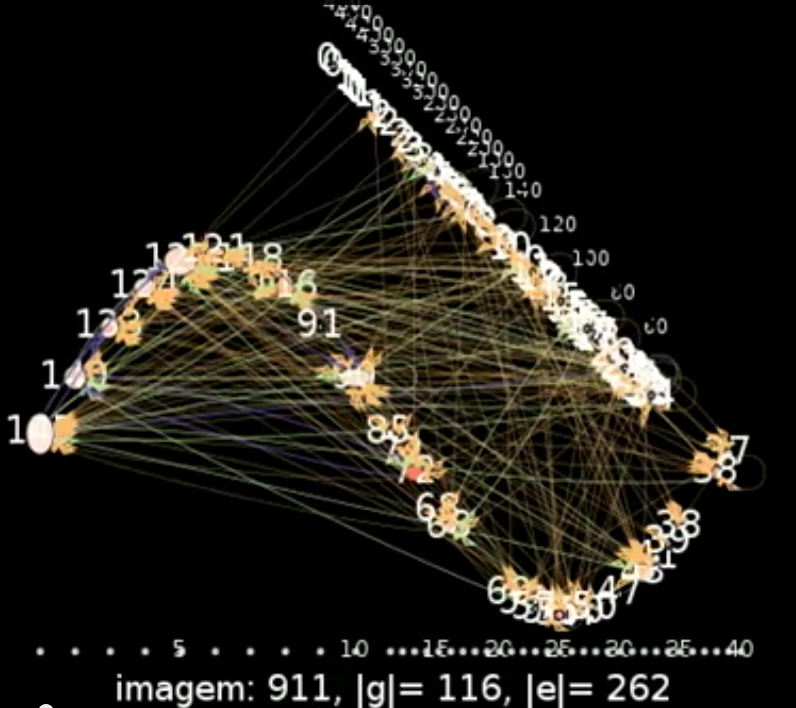
\includegraphics[width=.5\textwidth]{versinus_}
% \caption{A figure caption is always placed below the illustration.
% Please note that short captions are centered, while long ones are
% justified by the macro package automatically.} \label{fig1}
% \end{figure}

The parameters of the placement are:
\begin{itemize}
  \item the horizontal margin, i.e. the distance from the left border to the first hubs, assumed the same as the distance from the right border to last intermediary node.
  \item The amplitude of the sine segment.
  \item The positions $(x0,y0)$ and $(x1,y1)$, i.e. the endpoints of the segment for the peripheral sector.
\end{itemize}

\noindent Avoiding clutter with the hubs motivated both 
the positioning of the peripheral sector in the upper-right corner and
the placement of the most active peripheral nodes next to the intermediary sector, i.e. the ordering along the peripheral line.

\subsection{Drawing nodes, links and auxiliary information}
\subsection{Observation of the evolving network}

\section{Software implementations}\label{sec:imp}
\section{Insights gathered}\label{sec:ins}
\section{Conclusions and further work}\label{sec:con}
%
% ---- Bibliography ----
%
% BibTeX users should specify bibliography style 'splncs04'.
% References will then be sorted and formatted in the correct style.
%
\bibliographystyle{splncs04}
\bibliography{paperbib}
%
% \begin{thebibliography}{8}
% \bibitem{ref_article1}
% Author, F.: Article title. Journal \textbf{2}(5), 99--110 (2016)
% 
% \bibitem{ref_lncs1}
% Author, F., Author, S.: Title of a proceedings paper. In: Editor,
% F., Editor, S. (eds.) CONFERENCE 2016, LNCS, vol. 9999, pp. 1--13.
% Springer, Heidelberg (2016). \doi{10.10007/1234567890}
% 
% \bibitem{ref_book1}
% Author, F., Author, S., Author, T.: Book title. 2nd edn. Publisher,
% Location (1999)
% 
% \bibitem{ref_proc1}
% Author, A.-B.: Contribution title. In: 9th International Proceedings
% on Proceedings, pp. 1--2. Publisher, Location (2010)
% 
% \bibitem{ref_url1}
% LNCS Homepage, \url{http://www.springer.com/lncs}. Last accessed 4
% Oct 2017
% \end{thebibliography}
\end{document}
